Uno dei parametri più importanti che riguardano l'esito dell'analisi è il numero di componenti della base \(V'\) che vengono mantenute, le cosiddette "\textit{Componenti Principali}". Come spiegato in \ref{variance}, è possibile calcolare la varianza trattenuta in funzione del numero di componenti della base \(V'\):
\begin{figure}[H]
    \centering
    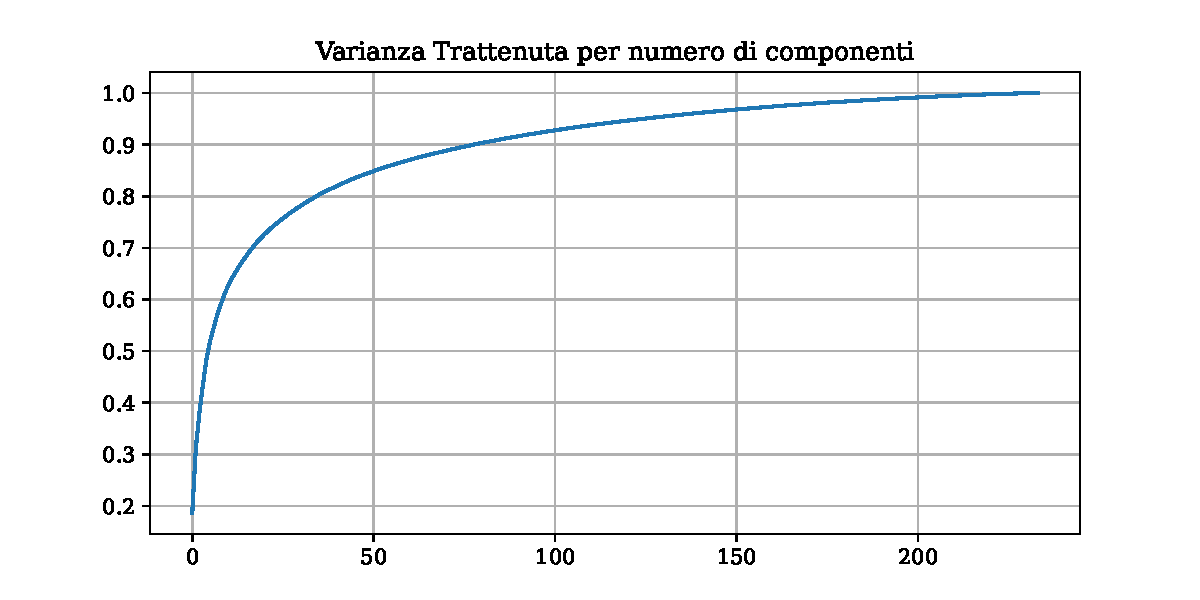
\includegraphics[scale = 0.7]{pictures/variance_cum.pdf}
    \caption{Varianza cumulativa in funzione delle componenti princpali}
    \label{cum_variance_graph}
\end{figure}
\noindent Come si evince dalla Figura \ref{cum_variance_graph}, per trattenere il \(70\%\) della varianza sono necessarie \(17\) componenti mentre per trattenerne il \(90\%\) ne sono necessarie ben \(78\). Sarà quindi interessante valutare l'accuratezza delle predizioni in funzione del numero di componenti principali utilizzate: ci si aspetta che un minor numero di componenti, sebbene trattengano meno varianza, rendano più snello il calcolo delle distanze a discapito dell'accuratezza. Al contrario, utilizzando un numero più elevato di componenti, le approssimazioni delle immagini risulteranno più accurate e ci si aspetta quindi un'accuratezza delle predizioni più elevata a discapito del tempo computazionale. 
\\
\\
Sono stati testati pertanto vari livelli di varianza trattenuta. Per ciascun livello risulta un numero di componenti principali trattenute diverso. Per ogni livello di varianza trattenuta è stata calcolata l'accuratezza delle predizioni. In Figura \ref{accuracy_vs_pc graph} un riassunto dell'esperimento.
\begin{figure}[H]
    \centering
    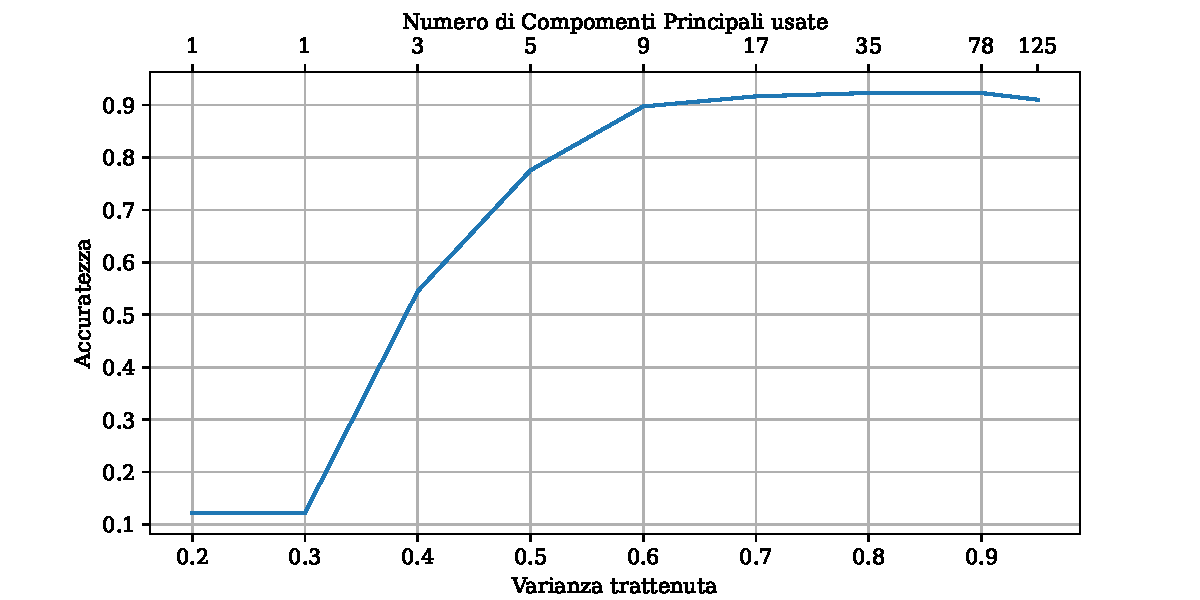
\includegraphics[scale = 0.7]{pictures/accuracy_vs_pcs.pdf}
    \caption{Accuratezza in funzione della varianza trattenuta e del numero di componenti principali usate}
    \label{accuracy_vs_pc graph}
\end{figure}
\noindent È interessante notare come utilizzando 125 componenti principali (corrispondenti al 95\% di varianza trattenuta) l'accuratezza scenda leggermente rispetto all'esperimento con 78 componenti principali. Questo fenomeno è probabilmente dovuto alla cosiddetta "\textit{curse of dimensionality}" per cui il concetto di "distanza" perde di significato in spazi di grandi dimensioni.
\\
\\
\noindent Tutti gli esperimenti sono stati eseguiti considerando una soglia di accettazione \(\Theta\) calcolata nel modo seguente:
\begin{description}
    \item[\(\bullet\)] Si esclude un soggetto \(s_N\) dal dataset (l'ultimo soggetto del dataset)
    \item[\(\bullet\)] si calcola la distanza di ciascuna immagine del soggetto dall'autospazio
    \item[\(\bullet\)] si calcola la media \(\theta\) sulle immagini di ciascuna distanza  
    \item[\(\bullet\)] si assegna \(\Theta = \gamma \theta\) dove \(\gamma\) è un valore di tolleranza settato su \(\gamma = 1.3\) 
\end{description}
\newpage
\subsection*{Visualizzazione dell'autospazio}
Un'interessante grafico è quello che ci permette di visualizzare l'autospazio. Utilizzando infatti 2 componenti principali ciascuna immagine può essere collocata su un piano cartesiano:
\begin{figure}[H]
    \centering
    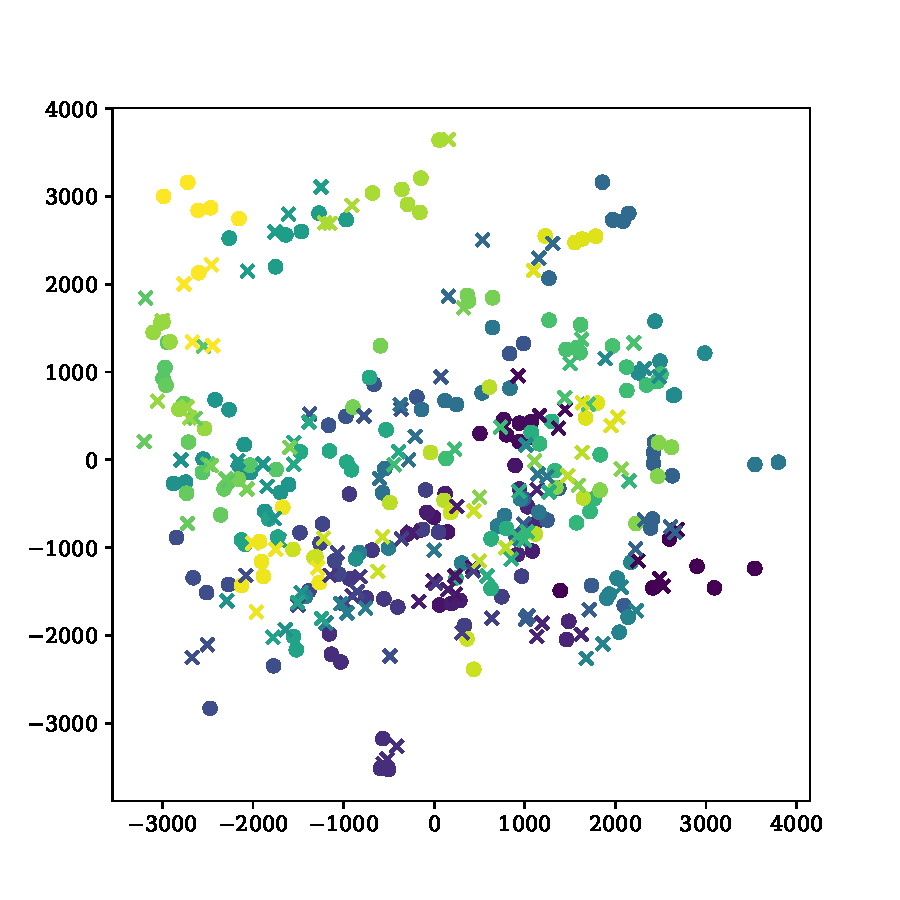
\includegraphics[scale = 0.7]{pictures/visualization.pdf}
    \caption{Rappresentazione 2D delle immagini. Le immagini rappresentate con marker "x" sono quelle utilizzate per il test mentre quelle con marker "o" sono le immagini di training. A colori diversi corrispondono soggetti diversi.}
    \label{visualization}
\end{figure}